\documentclass[10pt,draft, conference]{IEEEtran}


\usepackage{xcolor}

\newcommand\todo[1]{\textcolor{red}{#1}}

\title{How to win a star at GitHub}

\author{
    \IEEEauthorblockN{Michel Kraaijeveld}
    \IEEEauthorblockA{Delft University of Technology\\
                    Delft, the Netherlands\\
                    Email: \\}
    \and
    \IEEEauthorblockN{Tom den Braber}
    \IEEEauthorblockA{Delft University of Technology\\
                        Delft, the Netherlands\\
                    Email: t.d.denbraber@student.tudelft.nl}
}

\begin{document}

\maketitle
\IEEEdisplaynontitleabstractindextext

\begin{abstract}

\end{abstract}

\section{Introduction}
    More and more people make use of GitHub to host their Open Source Software (OSS)\cite{github-2013}. 
    GitHub is not only a place were people share their software, it has also become a `social network' for software developers because of its social features. \cite{dabbish-2012} 
    One of those social features is `starring' a project. Users can show their appreciation for a project by giving it a  star and many of GitHub's own rankings are also based on the amount of stars a project has.\cite{github-stars-2016} 
    Therefore one can state that the amount of stars gives an indication of how many people appreciate the project.
    
    However, there might be several factors that can be related to the amount of stars of a project. 
    One can think of the functionality that the project offers, but what about projects that offer more or less the same functionality but have a greatly different amount of stars? Other factors such as popularity of the topic of the project, it being easy to use, e.g. a library that can be added, and more, can all have influence.
    
    This paper will be looking at the stars given to OSS projects and whether certain factors are related to the amount of stars a project can possibly get, and if there are key points to focus on when aiming at having the most stars as possible.
    \todo{Extent introduction a little bit?}

    %\todo{
    %    \begin{itemize}
    %        \item What are stars?
    %        \item Why are stars cool?/what do they indicate?
    %        \item How is it possible to research them?
    %    \end{itemize}
    %}

%Uit 2011, maargoed toen al populair, dus tegenwoordig moeten zo nog wel meer hebben:
%https://github.com/blog/841-those-are-some-big-numbers
%https://github.com/blog/1204-notifications-stars

%%Popularity: (TODO: add more of those as actual references??)
%https://github.com/blog/1724-10-million-repositories
%https://github.com/blog/685-one-million-repositories
%http://readwrite.com/2011/06/02/github-has-passed-sourceforge

%%%Language popularity:
%https://github.com/blog/2047-language-trends-on-github
%https://www.researchgate.net/profile/Christophe_Giraud-Carrier/publication/228993701_Programming_language_trends_in_open_source_development_An_evaluation_using_data_from_all_production_phase_sourceforge_projects/links/0fcfd510c5d5b16f8a000000.pdf /???????

%http://www.iculture.nl/swift-populariteit-github-programmeertalen/
%https://www.githubarchive.org


\section{Problem Description}
    Although the amount of stars for a project are far from the only indicator of a project's success, they give an indication of how many people actually like the project.
    For developers, it might be important to know how they can gain the appreciation of other GitHub users: the more people that use or collaborate to a project, the faster it will evolve.

    We will now further concretize the subject of this research. 
    The main research question is as follows: `Can we predict the amount of stars a project on GitHub will get when looking at its characteristics?'
    This high-level question can be split up into two more concrete questions:
    \begin{itemize}
        \item Which factors influence the popularity of a project?
        \item To what extent can we accurately predict the amount of stars on a project?
    \end{itemize}
    
    %\todo{waarom onderzoeken hierin, waarom is het nuttig, wat hebben mensen eraan}\\
    
    To answer the questions specified earlier, a dataset which contains a lot of data concerning the projects on GitHub is needed. 
    This dataset is available: GHTorrent \cite{gousios-2013} is a dataset which is constantly mining the GitHub application for more data on projects, and contains all the data that we need for this research.

    %\todo{More background info}

    However, since it also contains data that is not useful for this particular research, we chose to create our own dataset based on GHTorrent.
    This dataset contains 2000 open source projects with several features defined for each of them and is freely available for anyone to use.
    It can \todo{(not yet)} be found on https://github.com/IN4334-group-1/msr.


    %\todo{
    %\begin{itemize}
    %    \item Motivation
    %    \item Our research questions
    %    \item a short introduction into the dataset of Gousios
    %\end{itemize}
    %}


\section{Methodology}
    Now that the research questions have been discussed, the approach for answering those questions can be explained.
    We will start by detailing our sampling method. 
    Thereafter, we introduce the features which we think are related to the amount of stars that a repository has.
    Lastly, we discuss the methods for actually constructing a learning model that we can use to predict the amount of stars for a given project.
    \subsection{Sampling Method}
        The distribution of stars per project appears to be extremely right skewed: there are projects with one or zero stars, while there are much less projects which have a lot of stars, as can be seen in Figure \ref{fig:nr-stars-plot}.
        Because of this skewness, the decision was made to use \textit{stratified sampling}\cite{TODO}.
        With stratified sampling, we first have to divide the population into strata. 
        Thereafter, we sample an equal amount of projects from each of these strata; 
        all these samples together form the sample that is being used in the rest of the project.
        Each stratum has as characteristic that the amount of stars of the project in that stratum fall within a certain range. 
        The ranges that will be used in this project are: [0, 10], (10, 100], (100, 1000], (1000, +].
        The reasoning behind these ranges is based on the research by Chen et al. where they used the same ones for splitting their data that was based on forks; as the same characteristics applied to the amount of stars. \ref{TODO}
        Because the dataset is very large, we can also create a quite large sample:         
        out of each stratum, we will randomly select 500 projects for each stratum. The total size of our sample will therefore consists of two thousand projects.
        
        Further, we split up our sample in a training set and a testing set. Out of our sample, we randomly pick half of the projects which will form our training set. The other half of the sample will be used as a testing set.
        
        Although we mentioned that the selecting of projects is completely random, it actually is not. To reduce bias in our sample, we decided to filter out any project by Google, Microsoft or Apple.
        The way in which they use GitHub is different from most other projects, but they do have a lot of stars, partly due to brand awareness; therefore, they are not included in our sample.
        Furthermore, deleted projects are also not contained in the dataset.
        The reason for this is that not all of the features can be successfully applied to deleted projects, and we don't consider them to hold the key to getting stars on GitHub; as we would expect a successful project to still be around.
        
        %\todo{
        %    \begin{itemize}
        %        \item Stratified sampling because of skewness
        %        \item Discuss strata intervals
        %        \item Discuss sample size
        %        \item Discuss items that are excluded from the sample (google/microsoft projects)
        %        \item Discuss training/testing split
        %    \end{itemize}
        %}
        
    \begin{figure}[t!]
        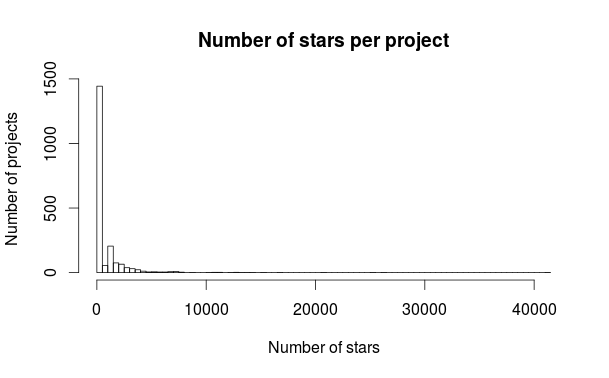
\includegraphics[width=250pt]{figures/number-of-stars-per-project}
	    \caption{The number of stars per project}
	    \label{fig:nr-stars-plot}
	\end{figure}
    
    \subsection{Features}
    To be able to predict the amount of stars an OSS project will get, a model need to be designed.
    Therefore a number of features is discussed first, which could be related to the amount of stars on a project.
    Each of these features fall into one of the high-level features that are specified: general project characteristics, popularity of developers or organisation, and activity.
    Next to these high-level features, the domain is also considered as that is another aspect that can be related to the amount of stars.
    After the features are defined, we can use them in combination with a machine learning algorithm to create the actual prediction model.\\

    \subsubsection{General project characteristics}
    The first high-level feature contains general features belonging to a project. 
    A feature is considered a general project feature if it cannot be categorized into the other high-level features.
    \begin{LaTeXdescription}
        %\item[Number of commits]
        %This is the total amount of commits since project creation.
        %A commit can either be an addition from one of the project developers, or a merge from an accepted pull request.
        %When the number of commits is larger, this might indicate that a project attracts more users.
        %TODO: Misschien number of commits er maar uit laten, hebben commits / day ook al
        \item[Project country of origin]
        The country of origin refers to the country in which the project was intially created.
        This can either be based on the developer that created the project, or on the majority of developers in the organisation
        \item[Number of commits per developer]
        The total amount of commits that each of the developers in the project have.
        These commits do not include merge commits.
        %TODO: check whether commits include merge commits or not!
        \item[Number of forks]
        The number of forks is the total amount of forks that the project got since its intial creation.
        Since forking a repository means that someone is interested and possibly want to make use of the project as a resource for their own developments, it can be a good indication of the amount of stars a project might possibly get.
        \item[Number of pull requests]
        This numerical variable contains information about how involved contributors are to the project: do they make a lot of pull requests or not?
        \item[Total amount of contributors]
        Someone is considered a contributor when he or she can directly commit to the repository (developer) or when a pull request is merged into the project (external-developer).
        When a project has more contributors, it might give a prediction on the amount of stars the project will possibly get.
        \item[Main programming language]
        The language that is used most throughout the project is considered the main programming language. 
        Since some languages are easier to learn and understand, or is more popular, projects that use that language might be able to attract more users and therefore stars.\cite{ieee-2015}
        \item[How long does the project exists]
        Newer project might have fewer stars, since they are not discovered by the majority of the GitHub users. 
        Therefore the time a project exists, might have influence on the amount of stars the project currently has.
        \item[Description available] GitHub offers the possibility of giving a one-line description, which is placed directly below the title. Having a good or catchy description might attract users to examine the project further.
        %\item[Number of bytes] \todo{Larger projects have more lines of code, which can give an indication of being actively maintained or having multiple contributors $->$ more chance to get stars?}
        %TODO: check whether number of bytes can be useful in model
    \end{LaTeXdescription}\hspace*{\fill}

    %name of the project
    %origin of project ('project owner'->country)
    %#commits
    %#commits/developer
    %amount of contributors on project
    %programming language
    %hoe lang bestaat het project al?

    \subsubsection{Characteristics of developers and organisation}
    When a developer or organisation is already known on GitHub and has established a group of followers, a new project created by them can get attention from other users more easily.
    To find out whether this has any relation to the amount of stars a project can possibly get, five features are created to be included in the prediction model.
    \begin{LaTeXdescription}
        \item[Average number of followers per developer]
        This is the average number of followers between all developers that contribute to the project.
        \item[Maximum number of followers per developer]
        This number indicates the maximum amount of followers the developers that contribute to the project have.
        \item[Number of developers in organisation]
        If the project is created by an organisation, this number indicates the amount of developers that belong to the organisation. Else, the number of developers in the organisation is set to be one.
        \item[Average number of followers per developer in organisation]
        If the project is created by an organisation, this number indicates the average amount of followers the developers in the organisation have. Else, the amount of followers of the project owner is inserted here.
        \item[Maximum number of followers per developer in organisation]
        This feature is like the previous one, except it now shows the maximum amount of followers a developer in the organisation has. When the project is owned by a user, the amount of followers of the project owner is inserted here.
    \end{LaTeXdescription}\hspace*{\fill}

    %--Developers
    %average #followers/developer
    %max #followers/developer
    %--Organisation
    %#developers
    %average #followers/developer
    %max #followers/developer

    %\todo{\subsubsection{Documentation} 
        %We also think that the fact that a project is not documented very well or even not documented at all can have influence on the appreciation users show for that project. Unfortunately, this is hard to measure as some projects do have extensive documentation on their own website, while they are not using the GitHub features for documenting the project.
        %At the moment of writing, it is also not possible to check if a project has a readme file or a wiki page on GitHub using the earlier discussed dataset. For future research, it might be interesting to involve this feature as well.}

        %TODO: move to future work
    %readme present?
    %wiki files present?

    \subsubsection{Activity}
        Another thing that we think can have an impact on the amount of stars a project gets, is the activity on that project: is it actively maintained or not?
    \begin{LaTeXdescription}
        \item[Number of commits per day]
            This numerical variable measures the average number of commits per day.
        \item[Ratio: accepted/total pull requests]
            This numerical variable contains the number of accepted pull requests divided by the total number of pull requests. It is also an indication of how `open' the project is.
        %\item[Number of releases]
        %    Although not all projects use the releases feature of GitHub, it is interesting to see if this numerical variable does have influence.
        %\item[Time between releases]
        %    This numerical variable is another measure of activity: it is the average time measured in days between each release for a given project.
       % \item[Number of branches]         \todo{not present in dataset}
    \end{LaTeXdescription}\hspace*{\fill}

    %#commits/day (follow-up: issue resolution time)
    %#releases 
    %#releases/time
    %#branches

 
    \subsubsection{Domain}
        Since some project domains are more popular, it is easier to get stars for projects in that domain, simply because more people are interested in that domain. \todo{references}
        Therefore the domain is also considered in the model, to make better predictions as features might weight different across domains.
        Unfortunately, the domain of a project cannot be automatically deduced from the dataset.
        Therefore, each project in our sample was given a domain manually.
        A domain is a categorical variable and is based on the 2012 ACM Classification. \cite{acm-2012}
        From this classification, we only considered the main categories.
        The reasoning behind this is that the amount of subcategories is quite large, and if the projects were divided into them there might be domains that would only contain a single project.


        %\todo{
        %    \begin{itemize}
        %        \item Discuss high level features
        %        \item Specify high level features into actual metrics
        %        \item Discuss adding of the `domain' to filter popular domain areas
        %    \end{itemize}
        %}
    
    
    \subsection{Finding relations}
        Now that the features have been listed, we can try to infer relations between those features. More specifically, we have an independent variable - the amount of stars for a project - and we will try to find relations with the independent variables - the features listed in the previous section.
        
        %The machine learning algorithm that first comes to mind is linear regression. However, some of our features are categorical, e.g. the programming language of a project, which makes it impossible to use linear regression.
        %Luckily, there is a variant available which is able to handle categorical variables; this algorithm is called `multiple linear regression'. 
        %Initially, this algorithm will be used. Depending on the results, we will try out other algorithms like random forest and naive bayes.
        
        %On top of the initial analysis using multiple linear regression, an attempt will be made to finetune our model so that the prediction is as accurate as possible. The step-wise regression algorithm will be used for this task.
        On beforehand, we obviously do not know how and if the data is related. Luckily, there are many learning algorithms available which can be used. 
        These algorithms take a model, which consists of a dependent variable and a list of features.
        The learning algorithm than takes this model and a set of data and tries to find a useful relation between the dependent variable and the independent variables.
        
        To find the relation between the features and the dependent variable, we will execute the following procedure for each of the algorithms that will be tried.
        \begin{itemize}
            \item Execute 10 times:
                \begin{itemize}
                    \item Split the dataset in a training and a testing set, both consisting of half of the data.
                    \item Train the model using the chosen learning algorithm and the training data.
                    \item Use the model to predict the amount of stars for the entries in the testing set.
                    \item Compare the predictions and the actual values, and calculate the $R^2$ value.
                \end{itemize}
            \item Compute the mean of all the $R^2$ values.
        \end{itemize}
        
        After this procedure, we have a reasonable estimation of how well the learning algorithm handles our dataset.
       %\todo{
       %     \begin{itemize}
       %         \item Discuss machine learning algorithms (Multiple Linear Regression, Stepwise regression)
       %     \end{itemize}
       % }

       %\todo{
       % \begin{itemize}
       %     \item Add machine learning algorithm info 
       %     \item Add how we created the feature table etc.?
       %     \item Add how we evaluate the machine learning algorithms (10 samples of our sample, calculate r-squared for each of them
       % \end{itemize}
       % }


\section{Results}
    \subsection{Initial Data Exploration}
	    \begin{figure}
	        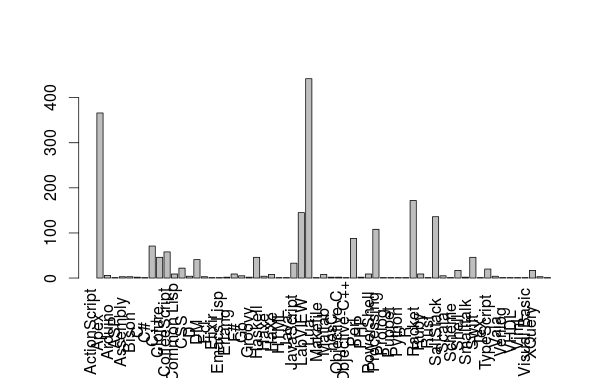
\includegraphics[width=250pt]{figures/language-frequency}
	        \caption{A histogram of the languages used in the projects}
	        \label{fig:language-frequency-plot}
	    \end{figure}	    
	    
	    \begin{figure}
	        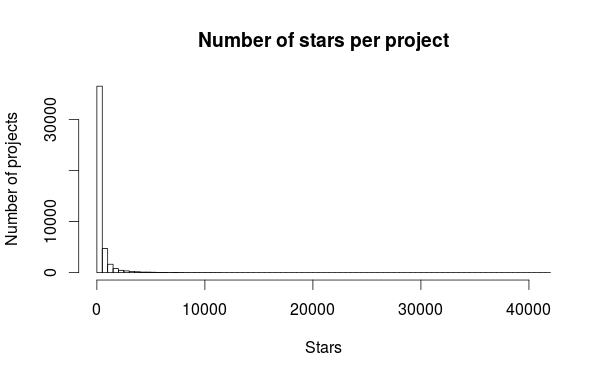
\includegraphics[width=250pt]{figures/star-distribution}
	        \caption{A histogram of the  number of stars per project}
	        \label{fig:star-distribution-plot}
	    \end{figure}
	    
	    \begin{figure}
	        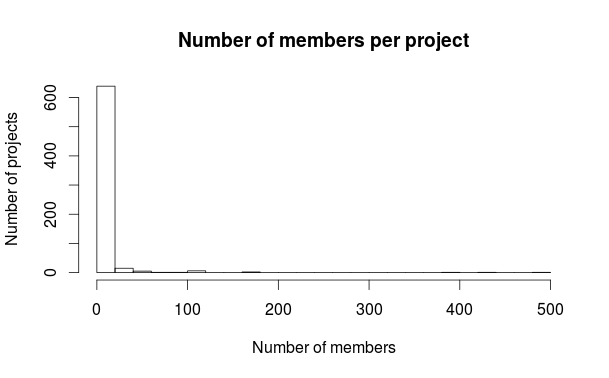
\includegraphics[width=250pt]{figures/number-of-members-per-project}
	        \caption{A histogram of the number of members per project}
	        \label{fig:number-of-members-per-project-plot}
	    \end{figure}
	    \begin{figure}
	        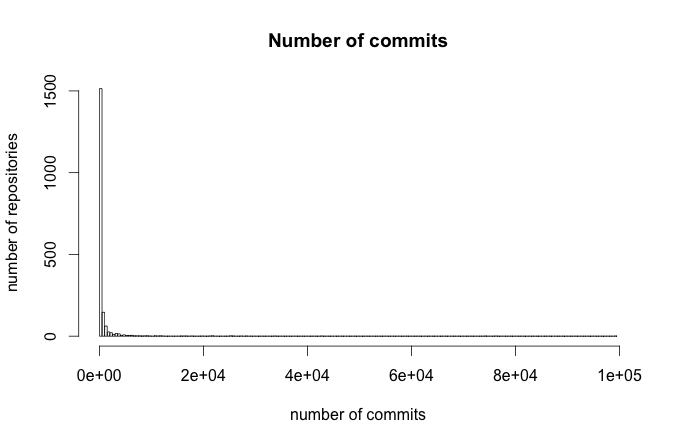
\includegraphics[width=250pt]{figures/number-of-commits-all}
	        \caption{A histogram of the number of commits per project}
	        \label{fig:number-of-commits-all-plot}
	    \end{figure}
	    \begin{figure}
	        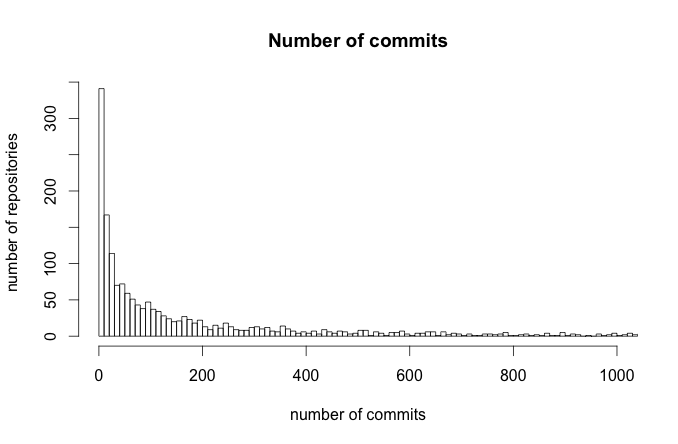
\includegraphics[width=250pt]{figures/number-of-commits-1000}
	        \caption{A histogram of the number of commits per project (with a maximum of 1000 commits)}
	        \label{fig:number-of-commits-1000-plot}

	    \end{figure}
    
    \subsection{Testing the model}
        \todo{Will be added later on, same for threats to validation}


\section{Related Work}
    Describe \cite{bissyande-2013}, \cite{chen-2014}, \cite{blincoe-2016}


\section{Conclusion}
	\todo{
	    \begin{itemize}
	        \item A brand new dataset with all kinds of nice features, freely available for everyone (ADD URL!)
	        \item The amount of stars can be predicted upto a certain extent. 
	        \item The main features used for this is the number of forks, the number of pull requests and the number of followers.
	    \end{itemize}
	}


\bibliography{references}{}
\bibliographystyle{ieeetr}

\end{document}
